\chapter{Conceitos Preliminares}
\label{cap:conceitos_preliminares}

\section{Algoritmos Genéticos}

Na década de 1960 John Holland inventou os Algoritmos Genéticos (AG) e os desenvolveu nos anos de 1960 e 1970 juntamente com seus alunos e colegas da Universidade de Michigan. E foi em 1975 através do lançamento de seu livro "Adaptation in Natural and Artificial Systems(1), que Holland apresentou os AGs à comunidade (5). Para Melanie (5), o objetivo original de Holland não era projetar algoritmos para resolver problemas específicos, mas sim estudar o fenômeno da evolução como ocorre na natureza, e desenvolver maneiras para que os mecanismos de adaptação natural pudessem ser importados para os sistemas computacionais.

Segundo \cite{linden12}, os algoritmos genéticos desenvolvidos inicialmente por Holland eram simples, mas conseguiam resultados satisfatórios para problemas considerados difíceis naquela época. Foi a partir de 1980 que os AGs começaram a evoluir, através da introdução de novas inovações e mecanismos cada vez mais elaborados, que tinham a intenção e necessidade de resolver, mesmo que aproximadamente, problemas práticos.

Os AGs utilizam muitas terminologias análogas às biológicas, porém suas entidades são muito mais simples do que as reais da biologia \cite{goldberg02}.
\begin{itemize}
\item Cromossomo:é a estrutura de dados que codifica uma solução para um problema, podendo ser uma cadeia de bits, ou um vetor com as variáveis de decisão do problema;

\item Indivíduo: é um membro da população, formado pelo cromossomo e sua aptidão;

\item População: é o conjunto de indivíduos de uma mesma espécie, e representa um conjunto de pontos candidatos a solução do problema;

\item Gene:para a biologia é a entidade de hereditariedade que é transmitida pelo cromossomo e que contém as características do organismo. Analogamente para os AGs é o parâmetro codificado no cromossomo;

\item Alelo: para a biologia representa uma das características alternativas de um gene. Para os AGs, representa os valores que um gene pode assumir;

\item Genótipo:para a biologia representa a composição genética, ou seja, o conjunto de genes de um indivíduo. Assim, nos AGs são representados pelas informações contidas no cromossomo;

\item Fenótipo:é o cromossomo decodificado, ou seja, é o organismo que pode ser construído a partir das informações do genótipo.Segundo \cite{linden12}, todos os AGs desenvolvidos para um determinado problema devem ter os seguintes elementos em comum:
\begin{itemize}
	\item 1. uma representação, em termo de cromossomo, para as soluções candidatas a resolução do problema;
	\item 2. uma maneira de se criar a população inicial;
	\item 3. uma função de avaliação, que permite ordenar ou classificar os cromossomos de acordo com a função objetivo;
	\item 4. operadores genéticos, que permitam alterar a composição dos novos cromossomos gerados pelos pais, durante a reprodução;
	\item 5. e valores para os parâmetros que os AGs usam: tamanho da população, taxa de crossover e taxa de mutação.
\end{itemize}
\end{itemize}

	

Em geral os AG também devem seguir um conjunto de passos, indicados na Figura adaptado de \cite{kondageski08}, onde cada ciclo completo, desde a avaliação de aptidão dos indivíduos, até a aplicação do operador de mutação, é considerado uma nova população. No decorrer do capítulo descreveremos com mais detalhes cada passo.

\begin{figure}[ht!]
	\centering
	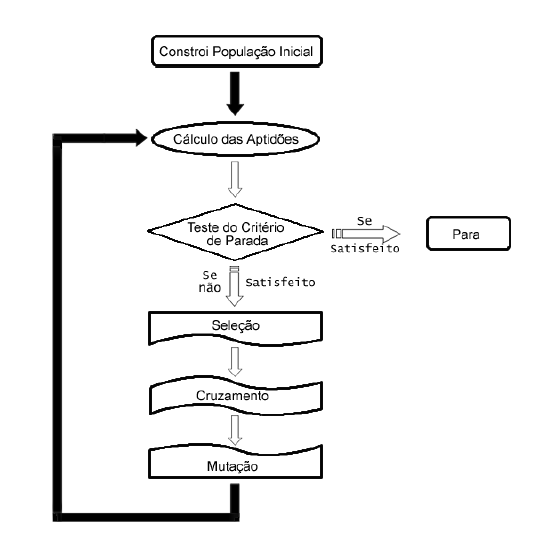
\includegraphics[scale=0.8]{figuras/processo-evolutivo.PNG}
	\label{processo-evolutivo}
\end{figure}

\subsection{Representação e Codificação}
 
 
Conforme vimos anteriormente todos os AGs devem possuir uma representação para as soluções candidatas a resolução do problema, chamada de cromossomo. Sua estrutura na maioria das vezes é um vetor, porém outras estruturas também podem ser utilizadas como árvores e matrizes. As codificações, ou representações mais utilizadas são a binária e a real.



Segundo \cite{linden12}, os primeiros cromossomos desenvolvidos por Holland em seus AGs utilizavam a codificação binária para representar os problemas. Apesar de esta codificação ser de fácil utilização e compreensão, em alguns casos obter a representação binária a partir do problema não é um processo muito óbvio, porém para um grande número de problemas de otimização esta representação é um processo natural. Devido a sua ineficiência em alguns problemas práticos com aplicações industriais, outras codificações surgiram como, por exemplo,a codificação com caracteres ou números reais.


\subsubsection{Representação Binária} 

Segundo \cite{mognon04} o código binário, que utiliza os símbolos 0 e 1 para representar as variáveis, é muito explorado para a codificação dos cromossomos. Na codificação binária os cromossomos são compostos por strings de zeros e uns, e os parâmetros (genes) são representados por conjuntos de bits. 

Porém, para \cite{catarina03}, quando a codificação binária é utilizada em problemas com variáveis contínuas e que se espera uma boa precisão na resolução, os cromossomos se tornam longos. Consequentemente este aumento dos cromossomos resultará também em um aumento de tempo para seu processamento.


\subsubsection{Representação Real}

Uma representação alternativa em problemas de optimização com variáveis ??contínuas de valor real é a representação cromossomo de ponto flutuante. Com esta representação, não há necessidade de um mecanismo de codificação explícita. Cada membro de cada população do algoritmo genético é um vetor de ponto flutuante. Os operadores genéticos (mutação e crossover) neste caso não lidar com cadeias de bits e são definidos de uma maneira diferente. Por exemplo, a operação de mutação não altera aleatoriamente um pouco, mas aleatoriamente escolhe um número de ponto flutuante dentro de um determinado intervalo.



\subsection{Criação da População Inicial}


A inicialização básica de um algoritmo genético clássico se resume à síntese de uma população inicial, sobre a qual serão aplicadas as ações dos passos subsequentes do processo. Tipicamente se faz uso de funções aleatórias para gerar os indivíduos, sendo este um recurso simples que visa a fornecer maior diversidade, fundamental para garantir uma boa abrangência do espaço de pesquisa \cite{goldberg02}. 

\subsubsection{inicialização de forma aleatória}

como o próprio nome já sugere, a população é gerada de forma aleatória, sem seguir nenhum padrão ou algoritmo. Pode ser considerado um método bom para testar o funcionamento de um AG, já que as soluções obtidas são puramente consequência da evolução dessa população aleatória, e não possuem interferência das características dos métodos utilizados para gerar a população inicial;

\subsubsection{inicialização heurística}

neste caso a população é gerada através de alguns métodos mais diretos como, por exemplo, o algoritmo guloso, inicialização randômica ponderada, ou mesmo uma inicialização gerada por um especialista no problema, sendo está forma muito utilizada especialmente em algumas aplicações industriais.

\subsection{Função de Avaliação}


Neste componente, todos os indivíduos da população 
sofrem um processo de avaliação, que visa a atribuição de um valor de adaptação para a solução do problema em estudo. Em conjunto com a escolha da representação, este é o ponto do algoritmo mais dependente do problema em si, pois é necessário que o AG seja capaz de responder sobre quão boa uma resposta é para o problema proposto por \cite{goldberg02}. 

Várias formas de avaliação são utilizadas: em casos de otimização de funções matemáticas, o próprio valor de retorno destas funções é aplicado ao indivíduo, e em problemas com muitas restrições, funções baseadas em penalidades são mais comuns. A função de avaliação é também chamada de função objetivo. 


\subsection{Operadores Genéticos}

Após a realização da avaliação dos indivíduos e a não satisfação do critério de parada, iniciase o processo de criação de uma nova geração, com a intenção de melhorar a aptidão dos indivíduos. Este processo de criação está fundamentado na aplicação dos operadores básicos deseleção, crossover e mutação, porém outros operadores podem ser utilizados e também variações destes considerados básicos. Nesta seção explicaremos melhor cada um destes operadores e seus principais métodos.


\subsection{Operador de Seleção}


Para que o processo de criação de uma nova geração inicie é necessário a seleção dos indivíduos que passarão para a nova geração, ou os chamados pais que irão gerar, através do crossover (reprodução), a nova geração. O operador responsável por essa classificação é o operador de seleção.



O operador de seleção assemelha-se ao processo de seleção natural, onde os indivíduos mais aptos, no caso de acordo com a função fitness , possuem uma probabilidade maior de serem selecionados. Contudo, a seleção não deve se basear apenas nos melhores indivíduos, pois estes podem não estar perto da solução ótima global, devendo também ser considerado os indivíduos com aptidão mais baixa, dando-lhes alguma chance de participar da reprodução \cite{mognon04}.


\subsection{Método da Roleta}

É um dos mais utilizados para a seleção dos indivíduos.  Neste método, cada indivíduo recebe uma porção da roleta de acordo com sua aptidão. Assim, consequentemente, os indivíduos com uma aptidão maior receberão também uma porção maior da roleta, o que aumentará sua probabilidade de ser selecionado.  Após as atribuições,  a roleta é girada e a porção sorteada corresponderá ao indivíduo selecionado, podendo ser girada quantas vezes forem necessárias de acordo com o número de indivíduos que se deseja para a próxima fase de cruzamento.

Para \cite{mognon04}, este método tem a vantagem de todos os indivíduos terem a chance de serem selecionados.  Entretanto, pode sofrer o efeito de dominância se algum indivíduo possuir uma aptidão alta em relação à média dos demais. A Figura  mostra um exemplo de configuração da roleta para uma população.

\subsection{Método de Torneio}


O primeiro passo desse método é a escolha de um subconjunto de indivíduos, que podem ser escolhidos aleatoriamente ou através de outro método, como por exemplo, o método da roleta. Esse subconjunto participará então do torneio, que consiste na competição dos indivíduos entre si considerando o seu valor de aptidão, ou seja, o vencedor será o indivíduo cujo valor de aptidão seja maior. Por fim, todos os membros do subconjunto são colocados novamente na população e o processo se repete, até que o número de indivíduos selecionados seja igual ao dos desejados \cite{mognon04}. 

\subsubsection{Operador de Crossover}

Após a seleção dos pais, um ou mais pares de indivíduos, o próximo passo para a geração dos novos indivíduos, os filhos, é a reprodução desses pares de indivíduos. O crossover é o operador responsável pela permutação do material genético dos pais durante o processo reprodutivo, permitindo assim que as próximas gerações, os filhos, herdem essas características. Este operador é aplicado seguindo-se uma taxa de crossover. O operador de crossover pode ser implementado de diversas maneiras, dentre elas as mais conhecidas são: crossover de um-ponto, crossover multiponto e crossover uniforme ou pontos aleatórios


\subsubsection{Operador de Mutação}
 
Este operador é necessário para que na nova geração possam ser inseridos novos materiais genéticos, ou seja, diversificar o material genético, como ocorre na natureza através de mutações ou anormalidades dos indivíduos. Por isso, este operador é aplicado levando-se em consideração a taxa de mutação , que geralmente é bem pequena. É muito simples de ser implementado: cada gene é analisado, através da probabilidade de mutação, para saber se aquela posição irá alterar seu valor ou não \cite{mognon04}.

\subsection{Parâmetros Genéticos}

Para que os algoritmos genéticos possam ser simulados se faz necessário a configuração de alguns parâmetros: tamanho da população, taxa de crossover e taxa de mutação. Segundo \cite{catarina03}, são esses parâmetros que afetam o desempenho dos AGs, desde um aumento do tempo de convergência, até uma convergência prematura ou mesmo a não-convergência para uma solução aceitável. No decorrer desta seção esses parâmetros serão descritos com mais detalhes, bem como suas influências


\subsubsection{Tamanho da População}


Este parâmetro determina o número de indivíduos que compõem cada população. Se a população for pequena, consequentemente a cobertura do espaço de busca do problema também será, o que poderá causar uma queda no desempenho do AGs. Assim, uma população grande resultará em uma cobertura maior do espaço de busca do problema, representando realmente o domínio do problema. Contudo, para se trabalhar com esta população maior, são necessários maiores recursos computacionais, ou/e um tempo maior de processamento do algoritmo \cite{catarina03}. Logo, este parâmetro deve ser ajustado de forma equilibrada, considerando os efeitos citados.

\subsubsection{Taxa de Crossover}


Representa a probabilidade com que ocorrerá o crossover dos indivíduos selecionados da população. Se a taxa for baixa, o algoritmo poderá se tornar muito lento, devido à inexistência de novos indivíduos. Quanto maior for esta taxa, mais rapidamente novas estruturas serão inseridas na população. Porém, se for muito alta poderá gerar efeitos indesejados, como a substituição da maior parte da população, o que poderá resultar na perda dos indivíduos de alta aptidão \cite{catarina03}.

\subsubsection{Taxa de Mutação}


Indica a probabilidade de ocorrer a mutação na população. Segundo Catarina \cite{catarina03}, se a taxa for baixa, ela previne que a solução fique estagnada em um valor, ou seja, a convergência prematura, e possibilita que se possa chegar em qualquer ponto do espaço de busca do problema. Se for uma taxa muito alta, tornará a busca essencialmente aleatória.
